\documentclass[problem]{mcs}

\begin{pcomments}
  \pcomment{FP_jections_nofunc}
  \pcomment{CH, S14}
  \pcomment{mashup of smaller problems}
\end{pcomments}

\pkeywords{
  composition
  surjection
  injection
  bijection
  total
  function
  infinite
}

%%%%%%%%%%%%%%%%%%%%%%%%%%%%%%%%%%%%%%%%%%%%%%%%%%%%%%%%%%%%%%%%%%%%%
% Problem starts here
%%%%%%%%%%%%%%%%%%%%%%%%%%%%%%%%%%%%%%%%%%%%%%%%%%%%%%%%%%%%%%%%%%%%%

\begin{problem}
Let $R: A \to B$ and $S: B \to C$ be binary relations such that $S
\compose R$ is a bijection and $\card{A} = 2$.

Give an example of such $R,S$ where neither $R$ nor $S$ is a function.
\iffalse Indicate exactly which properties---total, surjection,
function, and injection---your example of $R$ and your example of $S$
does \textbf{not} have.\fi

\hint Let $\card{B}=4$.

\begin{solution}
It is easy to see that $R$ must be total ($[\geq 1\ \text{out}]$) and
$S$ must be a surjection ($[\ge 1\ \text{in}]$).

$C$ must have 2 elements since $A \bij C$.

For the example with $R, S$ not functions, see Figure~\ref{fig:SoRbij}.

\begin{figure}

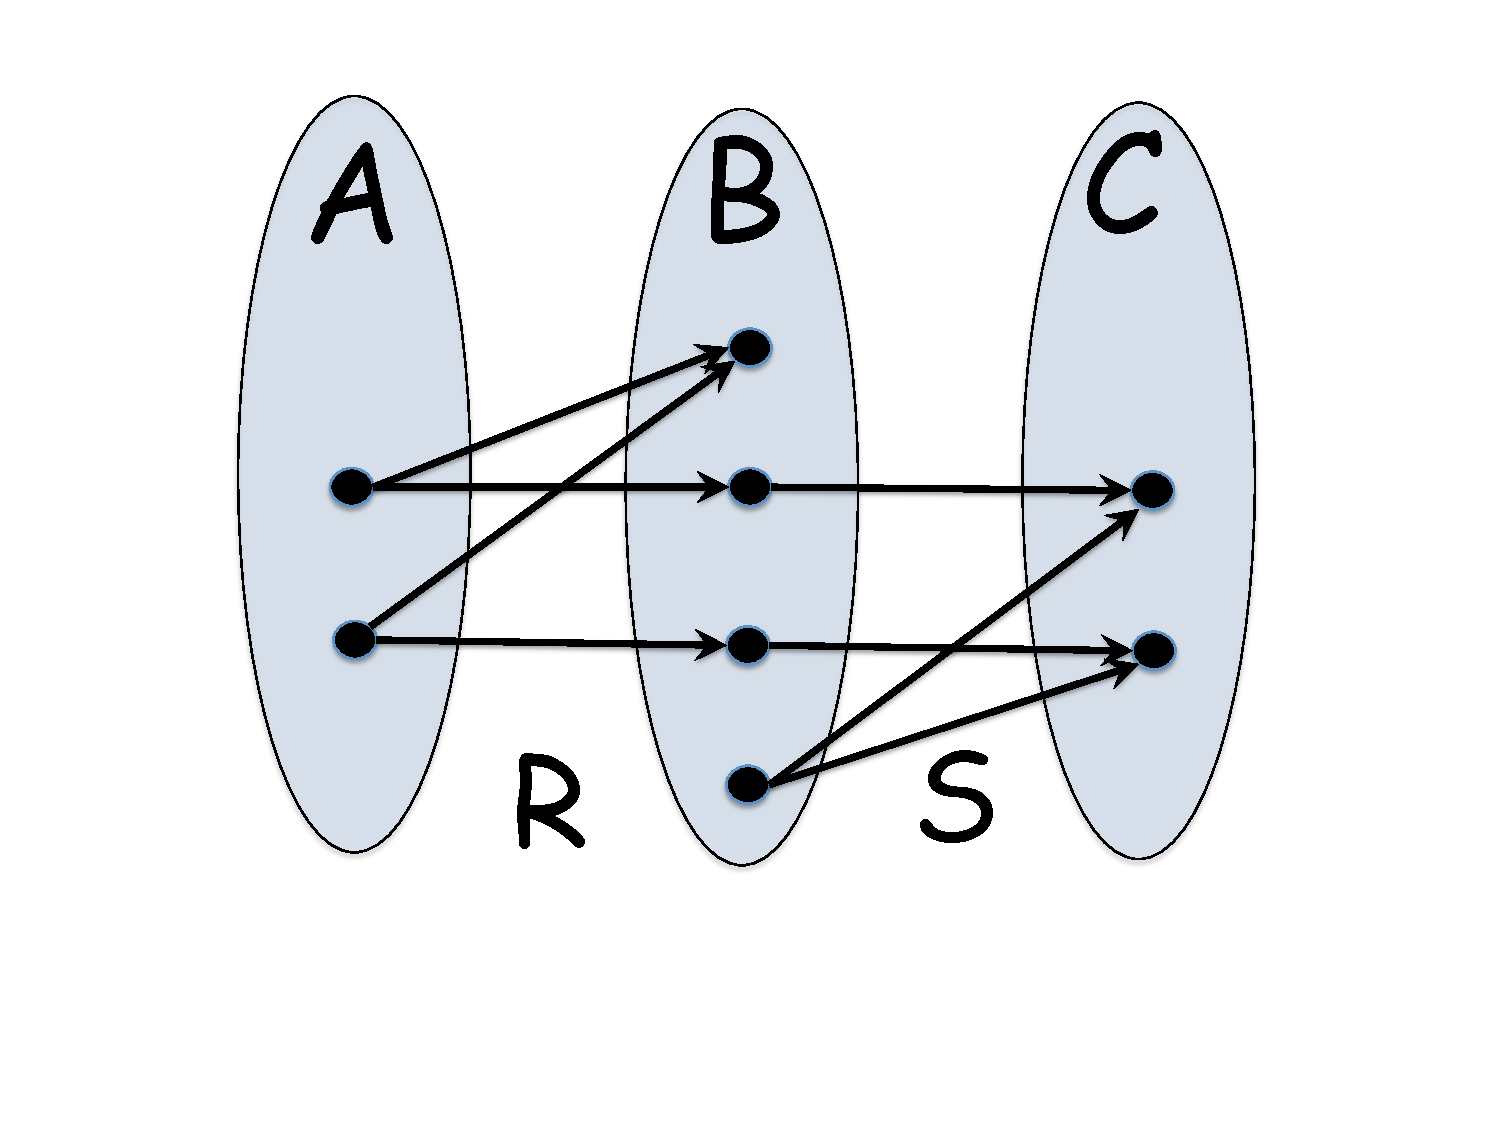
\includegraphics[width = 4in]{ScomposeR}

%\graphic{ScomposeR}

\caption{$S \compose R: A \to C$ is a bijection.}

\label{fig:SoRbij}

\end{figure}

Namely, let $\card{B} = 4$, and let there be an $R$-arrow from the
first element of $A$ to the second element of $B$ and an $S$-arrow
from this second element of $B$ to the first element of $C$; likewise
from the second element of $A$ to the third element of $B$ and from
this third element of $B$ to the second element of $C$.  These arrows
will provide the bijection defined by $S \compose R$.

Let the first element in $B$ have no $S$-arrow out and two $R$-arrows
in; so $R$ is not a function or an injection and $S$ is not total.
Let the fourth element of $B$ have two $S$-arrows out and no
$R$-arrows in; so $R$ is not a surjection and $S$ is not a function or
an injection.

So besides $R$ being total and $S$ a surjection, neither $R$ nor $S$
need have any additional ``jection'' properties. \iffalse That is,
\begin{itemize}

\item $R$ is not a function ($[\leq 1\ \text{out}]$), surjection,
  or injection ($[\leq 1\ \text{in}]$), and

\item $S$ need not be a function, total, or injection.

\end{itemize}
\fi

\end{solution}

\end{problem}

%%%%%%%%%%%%%%%%%%%%%%%%%%%%%%%%%%%%%%%%%%%%%%%%%%%%%%%%%%%%%%%%%%%%%
% Problem ends here
%%%%%%%%%%%%%%%%%%%%%%%%%%%%%%%%%%%%%%%%%%%%%%%%%%%%%%%%%%%%%%%%%%%%%

\endinput
